%%%%%%%%%%%%%%%%%%%%%%%%%%%%%%%%%%%%%%%%%%%%%%%%%%%%%%%%%%%%%%%%%%%%%%%%%%%%%%%%%%%%%%%%%%%%%%%%%%%
%%%%%%%%%%%%%%%%%%%%%%%%%%%%%%%%%%%%%%%%%%%%%%%%%%%%%%%%%%%%%%%%%%%%%%%%%%%%%%%%%%%%%%%%%%%%%%%%%%%
%%%%%%%%%%%%%%%%%%%%%%%%%%%%%%%%%%%%%%%%%%%%%%%%%%%%%%%%%%%%%%%%%%%%%%%%%%%%%%%%%%%%%%%%%%%%%%%%%%%
%%%%%%%%%%%%%%%%%%%%%%%%%%%%%%%%%%%%%%%%%%%%%%%%%%%%%%%%%%%%%%%%%%%%%%%%%%%%%%%%%%%%%%%%%%%%%%%%%%%

\chapter{Deterioro cognitivo y sueño}

En este capítulo se exponen varios temas para poder entender adecuadamente al sujeto de estudio (registros de PSG en adultos mayores), así como el contexto y la motivación para su estudio (el PDCL en adultos mayores).
%
Se responde, de manera muy breve, las siguientes preguntas:
\begin{itemize}
\item ¿Qué es el Deterioro Cognitivo Leve y cómo se diagnostica?
\item Clínicamente, ¿qué es el sueño y cómo se estudia?
\item ¿Cómo se relacionan el Deterioro Cognitivo Leve y el sueño?
\end{itemize}

Para simplificar la exposición, se considera al EEG como la técnica principal para el estudio de la actividad cerebral.
%
El lector interesado en una exposición más amplia sobre técnicas para el estudio del cerebro, puede referirse al libro \textit{``Medical Instrumentation. Applications and Design"} \cite{Webster}.
%
Con la misma intención de facilitar la lectura, se describe el sueño (desde el punto de vista clínico) antes de mostrar su posible utilidad como marcador para el DCL.

Si se desea revisar mayor información sobre los tópicos expuestos, pueden consultarse los libros \textit{``Guía para el diagnóstico neuropsicológico"} \cite{Ardila12} por Ardila y Ostrosky, y \textit{``Electroencephalography: Basic Principles, Clinical Applications, and Related Fields"} por Niedermeyer \cite{niedermeyer}.
%
Si se desean consultarse en mayor detalle los protocolos para registrar la PSG, o aquellos para clasificar las etapas de sueño, debe consultarse el Manual de la AASM \cite{AASM07}.
%
Para consultar con mayor detalle el proceso del sueño en sí, así como los procesos fisiológicos y psicológicos asociados, puede consultarse \textit{Psicofisiología del sueño} por Corsi-Cabrera \cite{Corsi1983}.

%%%%%%%%%%%%%%%%%%%%%%%%%%%%%%%%%%%%%%%%%%%%%%%%%%%%%%%%%%%%%%%%%%%%%%%%%%%%%%%%%%%%%%%%%%%%%%%%%%%
%%%%%%%%%%%%%%%%%%%%%%%%%%%%%%%%%%%%%%%%%%%%%%%%%%%%%%%%%%%%%%%%%%%%%%%%%%%%%%%%%%%%%%%%%%%%%%%%%%%

\section{Deterioro Cognitivo Leve}
\label{seccion:dcl}

El envejecimiento es determinado por una serie de procesos moleculares, celulares, fisiológicos y psicológicos que conducen directamente al deterioro de funciones cognitivas, específicamente atención y memoria \cite{Park09}.
%
Como consecuencia, los \textbf{adultos mayores} son especialmente propensos al deterioro cognitivo; por precisión, en lo siguiente se usará el término \textit{adulto mayor} para referirse a individuos con 60 o más de edad años.
%
Cabe destacar que la funcionalidad del adulto mayor no depende meramente de la edad, sino que está relacionada con el estilo de vida, los factores de riesgo, el acceso a la educación y las acciones para el cuidado de la salud realizadas en edades más tempranas \cite{Sanhueza14}.
 
La \textbf{demencia}, considerada como el estado más grave del deterioro cognitivo, es definida en el el Manual Diagnóstico y Estadístico de Trastornos Mentales (DSM-V, por sus siglas en inglés y la versión consultada) como sigue:
\begin{quote}
``Un síndrome que consiste en el desarrollo de déficit cognoscitivos suficientemente graves como para 
interferir significativamente en las actividades laborales y sociales, respecto al nivel de 
actividad previo.\\
%
Los sujetos con demencia tienen una baja capacidad para aprender información nueva y suelen olvidar 
lo aprendido anteriormente, siendo éste el síntoma más prominente."  \cite{DCM5}
\end{quote}

Se considera que la demencia es irreversible, y no se han identificado curas definitivas \cite{PlanAlzheimer04}. 
%
Debido a ello, ha surgido un gran interés en definir y diagnosticar sus etapas tempranas. 
%
El diagnóstico temprano es importante para un tratamiento adecuado que revierta o desacelere el avance de este síndrome \cite{Knopman01}.

Bajo esta línea de pensamiento se considera al \textbf{Deterioro Cognitivo Leve} (DCL) como una etapa precursora de la demencia, y que es definida como sigue: 
\begin{quote}
``Una alteración adquirida y prolongada de una o varias funciones cognitivas, que no corresponde a un 
síndrome focal y no cumple criterios suficientes de gravedad para ser calificada como demencia."
\cite{Robles02}
\end{quote}

Para fines de la definición anterior, se entiende por \textit{síndrome focal} al daño en una estructura nerviosa específica, cuya causa es conocida (como una hemorragia o una embolia) y cuyo inicio sea inmediato y evidente. 

El DCL puede detectarse por medio de diversos métodos, que pueden ser complementarios entre sí. 
%
La forma de detección más simple es la percepción de fallas en la memoria por parte del individuo u de otro. 
%
La percepción subjetiva del deterioro cognitivo \textit{esperado} por el envejecimiento provoca que esta forma de detección sea poco fiable.
%
Una alternativa más {formal} consiste en la entrevista clínica de un especialista, la aplicación de cuestionarios sobre dificultades en la memoria, o incluso al uso de pruebas neuropsicológicas. 

En psicología, los instrumentos de medición comunes son las \textbf{pruebas neuropsicológicas}, 
entendidas como muestras de alguna conducta de interés a las que se asignan puntajes para comparar 
cuantitativamente a los sujetos \cite{Ardila12}.
%
Se considera que a través de estas herramientas es posible declarar objetivamente las deficiencias cognitivas o conductuales de los individuos, así como su severidad y características.

De forma auxiliar para el diagnóstico del DCL, se pueden efectuar análisis genéticos, químicos, de imágenes cerebral, entre otros que estudien el sistema nervioso central.
%
Se espera que dichas técnicas, en combinación con las pruebas neuropsicológicas, permitirán diagnosticar más acertadamente el DCL y desentrañar los fenómenos neurobiológicos subyacentes.

Un referente ampliamente usado para el diagnóstico del DCL son los criterios para Alzheimer de la NINCDS--ADRDA, propuestos %en 1984 
por el \textit{National Institute of Neurological and Communicative Disorders and Stroke} y la \textit{Alzheimer's Disease and Related Disorders Association} \cite{McKhann,Dubois07}. 
%
Dichos criterios proporcionan protocolos para diagnosticar el Alzheimer y algunas enfermedades relacionadas (entre ellas el DCL), así como afecciones que generan síntomas similares. 
%
Desafortunadamente, las pruebas neuropsicológicas contempladas por los criterios de la NINCDS--ADRDA todavía no han sido \textit{validadas} en México, es decir que su efectividad para generar diagnósticos acertados no ha sido verificada para la población mexicana. 

Otra prueba neuropsicológica ampliamente extendida es el Mini-Mental State Examination (MMSE), propuesta por Folstein en 1975 \cite{folstein75} [citar mas, quiza??].
%
Sin embargo se ha reportado que, en la población mexicana, la prueba MMSE tiene baja sensibilidad para el diagnóstico de DCL en general, y baja especificidad para individuos con escolaridad muy baja o muy alta \cite{Ostrosky00}.
%
Para fines del comentario anterior, se entiende por \textit{sensibilidad} a la probabilidad de obtener verdaderos positivos, y por \textit{especificidad} a la probabilidad de obtener verdaderos negativos.

%En cambio, en estudios epidemiológicos, el Examen Cognitivo Transcultural (CCCE) y otras pruebas se han utilizado \cite{Rosales-Lagarde2016}. 
%%
%El CCCE muestra una prevalencia del 28.7 \% de deterioro cognitivo sin demencia (DCSD) que aumenta con la edad y disminuye con un nivel educativo más alto \cite{Mejia-Arango2011}. 

Una tercera opción, a la cual se ha dado gran peso en el presente trabajo, es la prueba neuropsicológica Neuropsi, desarrollada por Ostrosky y ?? en la Universidad Autónoma de México (UNAM) \cite{Ostrosky1999}.
%
La prueba Neuropsi ha sido validada para diversos grupos poblacionales en México, y se ha confirmado su utilidad para distinguir individuos con diverso grado de deterioro cognitivo.

En el contexto de la detección del DCL, es muy importante mencionar la \textbf{pseudodemencia depresiva}, una afección que no está relacionada con el deterioro cognitivo pero que puede generar un diagnóstico positivo para DCL.
%
De acuerdo al manual DSM-V, pseudodemencia depresiva se define como \textit{``un trastorno del afecto y que produce un aparente deterioro cognitivo"} \cite{DCM5}.
%
Bajo esta línea de pensamiento resulta conveniente decir que, como parte del diseño experimental, se han omitido participantes con síndromes focales, retraso mental, bipolaridad, esquizofrenia, entre otros trastornos de atención y memoria ajenos al deterioro cognitivo. 
%
Con base a ello, se omite una discusión más extensa de dicho tipo de afecciones; el lector interesado puede referirse al Manual DSM-V \cite{DCM5}.

\subsection{Probable Deterioro Cognitivo Leve}

En el presente trabajo se delimita al DCL por fines de precisión, usando para ello las pruebas neuropsicológicas. 
%
Se define operativamente el \textbf{Posible Deterioro Cognitivo Leve} (PDCL) como sigue:
\begin{quote}
``Una disminución significativa de las funciones cognitivas del sujeto con respecto las típicas de su edad y nivel de educación."
\end{quote}

Para fines de la definición anterior, el desempeño de las funciones cognoscitivas en un individuo es medido usando la prueba Neuropsi \cite{Ostrosky1999}; se considera que hay un déficit cognoscitivo \textit{significativo} si la puntuación obtenida es menor al umbral predefinido para su grupo de edad y nivel de escolaridad.
%
El umbral recomendado para la prueba Neuropsi debe calcularse como la media menos 3 desviaciones estándar de los puntajes típicos para individuos de cada grupo de edad y nivel de escolaridad; estos parámetros fueron estimados para la población mexicana por Ostrosky-Solís y colaboradores \cite{Ostrosky1999}.
%
En el cuadro \ref{anexo:neuropsi}, bajo la etiqueta \textit{Deterioro cognitivo} se recaban los \textit{puntajes de corte} usados para declarar el PDCL.

La palabra \textit{'probable'} en el PDCL hace alusión a que no constituye un diagnóstico \textit{irrefutable} del DCL.
%
En este sentido, el PDCL puede interpretarse como una condición \textit{necesaria pero no suficiente} para el DCL.

%%%%%%%%%%%%%%%%%%%%%%%%%%%%%%%%%%%%%%%%%%%%%%%%%%%%%%%%%%%%%%%%%%%%%%%%%%%%%%%%%%%%%%%%%%%%%%%%%%%
%%%%%%%%%%%%%%%%%%%%%%%%%%%%%%%%%%%%%%%%%%%%%%%%%%%%%%%%%%%%%%%%%%%%%%%%%%%%%%%%%%%%%%%%%%%%%%%%%%%

\subsection{Pruebas neuropsicológicas utilizadas}
\label{seccion:pruebas}

Dentro del contexto del presente trabajo, conviene describir las pruebas que fueron usadas para detectar el PDCL en adultos mayores.
%
Según la descripción que se dio del DCL, para efectuar su diagnóstico debe verificarse que el individuo cumpla las siguientes características:
\begin{enumerate}
\item Que presente un déficit en una o varias funciones cognitivas, pero que éste no cumpla los criterios suficientes para demencia.
\item Que los déficits cognoscitivos detectados no correspondan a síndromes focales,
\item Que el individuo no presente una afección que, sin estar relacionada con el deterioro cognitivo, genere síntomas similares.
\end{enumerate}
%
La condición 2 fue investigada mediante entrevistas con los participantes, constituyéndose como un criterio de exclusión.
%
Debido a la ausencia de excepciones, la condición 3 se limitó únicamente a detectar la pseudodemencia depresiva.
%
En conjunto, fueron usadas las siguientes pruebas:
\begin{itemize}
\item {Short Anxiety Screening Test (SAST)}\\ 
Evaluación corta para detectar trastornos depresivos y ansiosos. \cite{sinoff99}
%\cite{Vargas11}

\item {Geriatric Depression Scale (GDS)}\\
Evaluación corta para detectar cuadros depresivos en adultos mayores. \cite{Yesavage82}

\item {Mini--Mental State Examination (MMSE)}\\
Evaluación escrita relativamente rápida. Permite detectar el deterioro cognitivo, pero no proporciona \textit{muchos} detalles al respecto \cite{folstein75}. %\cite{Velasco15}

\item {Evaluación Neuropsicológica (Neuropsi)}\\
Evaluación extensiva sobre múltiples dominios. \cite{Solis03}

\item {Escala sobre las actividades cotidianas de la vida diaria (KATZ)}\\
Evaluación de la independencia del individuo para realizar tareas básicas de la vida diaria.\cite{katz70} \cite{Roumec14}
\end{itemize}

%%%%%%%%%%%%%%%%%%%%%%%%%%%%%%%%%%%%%%%%%%%%%%%%%%%%%%%%%%%%%%%%%%%%%%%%%%%%%%%%%%%%%%%%%%%%%%%%%%%
%%%%%%%%%%%%%%%%%%%%%%%%%%%%%%%%%%%%%%%%%%%%%%%%%%%%%%%%%%%%%%%%%%%%%%%%%%%%%%%%%%%%%%%%%%%%%%%%%%%

\section{Estudio clínico del sueño}
\label{capitulo:psg}

El sueño en el ser humano se considera como un estado de actividad, con propiedades características, y que influye de manera importante en la vigilia.
%
%Se suele definir al sueño en el ser humano como ``un proceso vital, con una estructura característica, y que presenta las siguientes propiedades" \cite{CarrilloMora}:
De manera operativa, puede caracterizarse según la siguientes propiedades \cite{CarrilloMora}:
\begin{enumerate}
\item Disminución de conciencia y reactividad a estímulos externos.
\item Fácilmente reversible, a diferencia de estados patológicos como estupor y coma
\item Inmovilidad y relajación muscular.
\item Periodicidad típica circadiana (diaria).
\item Los individuos adquieren una postura estereotipada.
\item La privación induce alteraciones conductuales y fisiológicas, las cuales se \textit{acumulan} en tanto persista la privación de sueño.
\end{enumerate}

La duración del sueño es determinada en gran parte por la edad; el recién nacido duerme entre 14 y 
18 horas, el lactante entre 12 y 14 horas, el niño en etapa escolar entre 11 y 12 horas y en la 
edad adulta, la mayoría duerme entre 7 y 8 horas \cite{Contreras13}.
%%
%%Paralelamente el sueño no es un proceso homogéneo, sino que tiene una estructura por etapas con 
%%rasgos fisiológicos distintivos.

En 1953 Asierinsky y Kleitman reportaron que existen patrones de actividad cerebral marcadamente diferentes durante el sueño, para lo cual usaron la técnica de electroencefalografía (EEG) \cite{Aserinsky}.
%
Con base a ello, el sueño se divide tradicionalmente en las etapas N y R, también referidas como NMOR y MOR; dichas etapas se distinguen en cuanto cómo se ve el EEG registrado en dichas etapas, así como los procesos fisiológicos que se llevan a cabo en el cerebro.
%
%En la siguiente sección se describe qué es el EEG y cómo se registra.
Por simplicidad expositiva, se describen primeramente las características de las fases de sueño según los criterios de y posteriormente se describe el EEG en sí. 
%
Las características descritas corresponden, muy a grosso modo, a los criterios establecidos por la \textit{American Society of Sleep Medicine} (AASM) \cite{AASM07}; en el cuadro \ref{cuadro:aasm} puede encontrarse una exposición más concreta y apegada al Manual de la AASM.

Durante la \textbf{fase R} el tono muscular disminuye, excepto para los músculos respiratorios y 
los esfínteres;
%
por \textit{tono muscular} se entiende a la contracción pasiva de los músculos durante el reposo, la cual permite una respuesta voluntaria rápida.
%
En esta fase de sueño las frecuencias cardíaca y respiratoria se vuelven irregulares. 
%
El individuo exhibe Movimientos Oculares Rápidos (MOR), en base a lo cual la fase R es conocida como \textbf{sueño MOR}.
%
En el EEG, aparecen ondas rápidas de bajo voltaje, irregulares, y que recuerdan la actividad durante al estado de alerta. 
%
Estos patrones de actividad cerebral no interrumpen el sueño sino que, contrariamente, incrementan el umbral para estímulos externos (qué tan fuerte debe ser un estímulo para afectar al individuo), motivo por el cual esta fase también es referida como \textbf{sueño paradójico}.
%
Cabe mencionar que durante la fase R se producen la mayoría de las ensoñaciones (referidas coloquialmente como \textit{sueños}), y que la mayoría de los pacientes que despiertan durante esta fase suelen recordar vívidamente el contenido de sus ensoñaciones \cite{Rosales14}.

%Para su estudio, el sueño se divide en dos etapas: N y R.
%
La \textbf{fase N}, se caracteriza por movimientos oculares lentos, tono muscular que decrece 
constantemente, actividad cerebral que recuerda al reposo, y la presencia de husos de sueño y 
complejos K. 
%
En base a la mayor o menor presencia de estas características, se definen las sub-fases N1, N2, N3.
%
Tradicionalmente se le refiere como \textbf{sueño no-MOR} (o NMOR).

\begin{table}
\caption[Criterios para la clasificación de etapas de sueño]
{Criterios para la clasificación de etapas de sueño según la AASM}
\centering
{\small
\begin{tabular}{lllll}
\toprule
&&   & Movimientos & Tono \\
\multicolumn{2}{l}{Etapa de sueño}& Características del EEG & oculares & muscular \\
\midrule
 W  & Vigilia & {Ritmo alfa} en $>50$\% de la época en   & No & Alto \\
    &         & la región occipital                &    &      \\
 N1 & NMOR 1  & Cambio de alfa por AABFM, atenuación & Lentos & $<$W     \\
    &         & del ritmo dominante. Ondas agudas   &    &      \\
 N2 & NMOR 2  & Husos de sueño y complejos K en la    & No & $<$W, $>$R     \\
    &         & primera mitad de la época. AABFM &    &     \\
 N3 & NMOR 3  & {Ondas lentas} (0.5--2 \hz, $>75$ \mv) en& No & $<$N2, $\approx$R \\
    &         & $>20$\% de la época. Husos de sueño       &&      \\
 R  & MOR     & Actividad baja amplitud y frecuencias & Rápidos & Bajo  \\
    &         & mixtas. Ondas agudas             &       &       \\
\bottomrule
\multicolumn{4}{l}{AABFM=Actividad de Amplitud Baja y Frecuencias Mixtas.}
\end{tabular}\\
}
\label{cuadro:aasm}
\end{table}

%%%%%%%%%%%%%%%%%%%%%%%%%%%%%%%%%%%%%%%%%%%%%%%%%%%%%%%%%%%%%%%%%%%%%%%%%%%%%%%%%%%%%%%%%%%%%%%%%%%

\subsection{Electroencefalografía}
\label{sec:eeg}

%\section{Fisiología}
%
%El registro de la actividad eléctrica en el cerebro, referido como \textbf{electroencefalograma} 
%(EEG), está tradicionalmente relacionado con la exploración de procesos mentales y sus trastornos; 
%como ejemplo se puede citar que Hans Berger, reconocido como el inventor del EEG, reportó usar 
%dicha técnica en 1932 para estudiar posibles cambios en un paciente con Alzheimer 
%\cite{historia_eeg}.
%
%El mecanismo base para la propagación de campos eléctricos en las neuronas, depende de la 
%capacidad de la membrana celular para mantener un equilibrio estable de iones con el medio 
%extracelular.
%%
%Dicho fenómeno fue ampliamente estudiado por Hodgkin y Huxley y puede describirse brevemente de la 
%siguiente manera: cuando existe un desequilibrio puntual y súbito en la concentración extracelular 
%de iones, se bombean iones a través de la membrana para restablecer el equilibrio en tal punto; 
%esta acción genera desequilibrios secundarios en regiones vecinas de la membrana, que a su vez 
%activan mecanismos similares. 
%%
%Como consecuencia, la perturbación en el potencial de membrana se propaga a lo largo de ésta y se 
%genera la transmisión de impulsos nerviosos en neuronas.
%%
%Un excelente referente sobre el tema es el libro por Ermentrout \cite{Ermentrout10}.
%

La técnica de electroencefalografía (EEG) consiste en medir la actividad postsináptica (transmisión de impulsos) entre neuronas en la corteza cerebral, lo cual se logra mediante electrodos colocados en el cuero cabelludo.
%
La corteza cerebral es la capa más exterior del cerebro, está formada por una fina capa de neuronas piramidales (denominadas así por su forma) altamente conectadas entre sí.
%
Típicamente se asocia a la corteza cerebral con las funciones cognitivas superiores \cite{niedermeyer}.
%
Conviene enfatizar que el término EEG usualmente se usa para referirse a registros hechos mientras el paciente realiza alguna actividad o se encuentra despierto y en reposo; el registro del EEG durante el sueño, adicional al registro de otras señales, es referido como polisomnografía.

%%, de modo que constituye una medida del la \textit{cantidad} de actividad cerebral. 
%%
%La actividad registrada en el EEG consta principalmente de la actividad postsináptica de las 
%neuronas piramidales en la corteza cerebral; éstas se encuentran altamente conectadas entre sí y
%forman capas densas.

Usualmente los registros de EEG muestran una actividad oscilatoria continua y cambiante, su frecuencia se considera entre 0.5 y 100 \hz. 
%
Su composición está fuertemente relacionada con el grado de actividad mental, mostrando diferencias claras durante vigilia y sueño, o durante quietud y concentración \cite{Clark98_2}.
%
Aunque el EEG es irregular la mayor parte del tiempo, suele mostrar patrones relativamente 
organizados, conocidos como \textbf{ondas cerebrales}; de forma tradicional, éstos se dividen en cinco grupos (referidos como \textbf{bandas}) según su\textit{frecuencia}:
\begin{itemize}
\item Delta, 0.5--3.5 \hz
\item Theta, 3.5--7 \hz
\item Alfa, 7--12 \hz
\item Beta, 12--30 \hz
\item Gamma, 30--100 \hz
\end{itemize}

Conviene destacar que diferentes autores han usado límites ligeramente diferentes para las bandas; de la misma forma algunos autores han incluido o excluido bandas, así como subdivisiones de éstas.

Adicionalmente a las ondas cerebrales, en el EEG pueden encontrarse \textit{eventos} visiblemente diferentes de su entorno, con%, referidos bien como  \textbf{paroxisomas}. 
%
%Los paroxisomas tienen 
una duración corta ($<1$ s) y \textit{formas} características.
%
Dos ejemplos importantes son los \textbf{husos de sueño} y los \textbf{complejos K}, definidos de manera visual y por su contexto fisiológico \cite{AASM07}; ambos tipos de ondas son típicos del sueño profundo y son usados para distinguirlo, aunque no se consideran ritmos ni pertenecen a las \textit{bandas} descritas anteriormente.
%
En la figura \ref{ritmos} se representa un arquetipo visual de cada una de las bandas, incluyendo los husos de sueño y complejos K.

\begin{figure}
\centering
\includegraphics[width=0.95\linewidth]{./img_diagramas/ondas_britannica.jpg} 
\caption[Ejemplos de ondas cerebrales encontradas en el EEG]
{Ejemplos de ondas cerebrales encontradas en el EEG durante el sueño. Imagen tomada de Encyclop{\ae}dia Britannica, 
versión en línea \cite{Britannica}.}
\label{ritmos}
\end{figure}

%\begin{table}
%\centering
%\caption{Generalidades sobre ondas cerebrales}
%{\small
%\begin{tabular}{lclll}
%\toprule
%Tipo de onda & Frecuencia [\hz] & {Ubicación usual} & {Condiciones usuales} \\
%\midrule
%Delta & 0.5 -- 3.5 &         & Síndromes focales. Sueño \\
%      &            &         & profundo en infantes \\
%Theta & 3.5 -- 7   & P, T    & Durante estrés emocional \\
%      &            &         & En infantes \\
%Alfa  & 7 -- 12    & F, P, O & Vigilia en reposo con \\
%      &            &         & ojos cerrados \\
%Beta  & 12 -- 30   & P, F    &      Actividad mental en\\
%      &            &         & adultos \\
%Gamma & 30 -- 100  &         &\\
%      &            &         & \\
%\midrule
%{Husos de} &&&\\
%sueño &&& \\
%{Complejo K} &&&\\
%&&& \\
%\bottomrule
%\end{tabular}\\
%Se abrevian los lóbulos cerebrales: F=frontal, P=parietal, T=temporal, O=occipital.
%}
%\label{tabla_ondas}
%\end{table}

Para realizar el registro del EEG en una forma estandarizada y comparable, deben indicarse los lugares donde se colocan los electrodos y la forma en que éstos están conectados.
%
En el contexto del presente trabajo, los electrodos fueron ubicados usado las coordenadas del \textbf{Sistema 10--20} \cite{Klem99}.
%\cite{Jasper58,Klem99}.
%
En dicho sistema los sitios se ubican en una \textit{cuadrícula} de distancias relativas (medidas en porcentajes), construida respecto puntos del cráneo relativamente fiables entre individuos:
\begin{itemize}
\item El \textit{inion}, un abultamiento en la región posterior del cráneo.
\item El \textit{nasión}, la unión del hueso frontal y los huesos nasales del cráneo.
\item El \textit{punto preauricular}, arriba del cartílago \textit{tragus} que protege el canal auditivo.
\end{itemize}

Aunque es perfectamente posible describir textualmente la construcción de las coordenadas en el sistema 10--20, se consideró que es más sencillo mostrarlos gráficamente en la figura \ref{img1020}.
%
En la misma imagen se muestran, de forma esquemática, los lóbulos de la corteza cerebral que dan nombre a las locaciones en el sistema: FP=fronotpolar, F=frontal, T=temporal, P=parietal, O=occipital.
%
Si bien no existe un lóbulo central, los electrodos `C' se suelen asociar al surco central; de forma similar, los electrodos `A' corresponden a los lóbulos auriculares, los cuales no tienen una actividad eléctrica importante y suelen usarse como referencia neutral.
%
Los electrodos se etiquetan con números pares en el lado izquierdo, números pares en el derecho y `Z' en el eje central.

\begin{figure}
\centering
\includegraphics[width=\linewidth]{./img_diagramas/cabeza_proporcionada_color_v4.pdf} 
%\vspace{2em}
\includegraphics[width=\linewidth]{./img_diagramas/cerebro_1020_v5.pdf} 
\caption[Colocación de electrodos según el sistema 10--20]{Colocación de electrodos según el sistema 10--20. \textbf{A.} Los electrodos se colocan en una malla de longitudes relativas (medidas en porcentajes) respecto a tres puntos de referencia: inion, nasion, punto preauricular.
%; los números impares se ubican a la izquierda, los pares a la derecha y se usa la Z para el eje central. 
%En el montaje ilustrado se usan como referencia neutral a los lóbulos de las orejas, electrodos cortocircuitados A1 y A2. 
\textbf{B.} División de la corteza cerebral en lóbulos, mostrando a grosso modo qué regiones son registradas usando el EEG. Los electrodos del sistema son referidos según los lóbulos cerebrales que \textit{representan}: Frontal, Temporal, Parietal, Occipital. Adicionalmente se registra cerca del surco Central, y los lóbulos Auriculares que son usado como puntos con actividad eléctrica negligible.
%\textbf{C.} Representación esquemática de los electrodos en el sistema 10--20, añadiendo los electrodos para actividad ocular y muscular. Se usarán diagramas en base a éste para reportar resultados.
}
\label{img1020}
\end{figure}

Para hablar sobre la forma en que se conectan lo electrodos entre sí, se denota a un par de electrodos como una \textbf{derivación} (también referida como \textit{canal}), mientras que el conjunto de derivaciones es un \textbf{montaje}.
%
En el contexto del presente trabajo se utilizó un montaje \textit{monopolar} (o también llamado \textit{referencial}) en cual se forman las derivaciones conectando en paralelo a cada electrodo con su respectivo electrodo auricular.

Es importante mencionar que las neuronas en la corteza cerebral tienen orientaciones muy diversas y que disparan de manera asíncrona, de modo que un periodo de gran actividad cerebral bien puede ser visto en el EEG como una actividad desorganizada y de baja amplitud.
%
En otra perspectiva, el cerebro se encuentra cubierto por las capas meninges, por el líquido encefalorraquídeo, el cráneo y el cuero cabelludo; en suma, los campos eléctricos generados en la corteza cerebral son \textit{víctimas} de una gran difusión espacial.
%
Es por ello que las señales captadas por los electrodos deben ser amplificadas analógicamente antes de ser registradas digitalmente.
%%
%A ello hay que añadir la difusión generada por las meninges, el líquido encefalorraquídeo y el 
%cráneo.

Un efecto colateral de amplificar la señal es la inclusión de \textbf{ruido}, entendiendo con ello a las señales que son registradas de manera no deseada.

Por ejemplo, los músculos faciales generan campos eléctricos con una frecuencia aproximada de 100 \hz; este tipo de ruidos \textit{persistentes} (referido como \textit{ruido de fondo}) son eliminados usando filtros de banda.
%
En contraparte, los ruidos esporádicos de corta duración, típicamente son señalados \textit{a mano} y provocan que el segmento de registro sea invalidado; por ejemplo, el deslizamiento de un electrodo en el curo cabelludo.

%; como ejemplo, pestañear 
%voluntariamente durante un episodio de quietud mental interrumpe las ondas alfa por cerca de dos 
%segundos. 

Como comentario, cabe mencionar que es posible usar electrodos colocados en otras zonas del cerebro, lo cual conlleva a técnicas similares con nombres diferentes; por ejemplo el electrocorticograma obtenido directamente de la corteza cerebral.
%
Así mismo, se menciona que el término EEG suele usarse independientemente de la cantidad y posición de electrodos usados para el registro: se pueden usar sólo algunas derivaciones del sistema 10--20, se pueden hacer cambios como el uso de la nariz como referencia neutral, o se pueden añadir más electrodos como en el sistema 10--10 \cite{Klem99}. 

%%%%%%%%%%%%%%%%%%%%%%%%%%%%%%%%%%%%%%%%%%%%%%%%%%%%%%%%%%%%%%%%%%%%%%%%%%%%%%%%%%%%%%%%%%%%%%%%%%%

\subsection{Polisomnografía}
\label{sec:emg_eog}

La técnica de polisomnografía (PSG) consiste en el registro simultáneo durante el sueño de múltiples variables \textit{variables fisiológicas} como respiración, ritmo cardíaco, temperatura, entre otros.
%
La decisión sobre las señales que componen la PSG depende del problema específico que será estudiado.
%
%En el contexto del presente trabajo conviene destacar 
%
Para ayudar en la clasificación de etapas de sueño, en el contexto del presente trabajo se usó una PSG con registros de actividad ocular, tono muscular y actividad cerebral (EEG).

%En el estudio por Vázquez Tagle y colaboradores, el registro de PSG incluyó registros de actividad 
%ocular (\textbf{electrooculograma}, EOG) y tono muscular (\textbf{electromiograma}, EMG), según las 
%recomendaciones de la AASM para clasificar las etapas de sueños. La ubicación estos últimos 
%electrodos es ilustrada en la figura \ref{emg_eog}.

La actividad ocular es registrada usando la electrooculografía (EOG), una técnica que explota el comportamiento dipolar del ojo con polos en la retina y la pupila; los movimientos del ojo producen variaciones en los campos eléctricos que pasa por él.
%
El registro del EOG incluye una derivación para cada ojo, LOG y ROG, cada cual formada por un electrodo y el electrodo auricular de referencia común.
%
Así como con el EEG, la ubicación de los electrodos para EOG se indican en la figura \ref{emg_eog}.
%
%El electrodo derecho se ubica 1 cm arriba y 1 cm a la derecha del rabillo derecho de ese ojo, mientras que el izquierdo tiene una posición similar pero debajo del ojo izquierdo; para una mejor explicación ver la figura \ref{emg_eog}.
%
Cabe mencionar que el registro de EOG debe ser interpretado como el movimiento del ojo, proyectado sobre el eje formado por los electrodos de registro.

El tono muscular es vigilado usando la técnica de electromiografía (EMG), la cual \textit{observa} la actividad eléctrica producida por las fibras musculares.
%
Su registro contempla 
%una derivación diferente al resto del PSG, pues contempla 
una derivación (EMG) con tres electrodos que actúan eléctricamente como tierra, fase y neutro;
%
la ubicación de estos electrodos se indica en la figura \ref{emg_eog}.
%
En el contexto del presente trabajo, más que analizarse la actividad muscular, se espera observar la \textit{desaparición} del mismo  durante el sueño MOR.
%
% el tono muscular corresponde a la contracción constante y pasiva (sin movimiento) de los músculos, siendo característica su \textit{desaparición} durante el sueño MOR.
%
%Los registros de EMG (canal EMG) admiten una interpretación más \textit{sencilla}, ya que los
%músculos son activados directamente por señales eléctricas: el tono muscular es la actividad 
%muscular basal, y se relaciona con la velocidad con que los músculos pueden \textit{salir} del 
%reposo.

A modo de comentario, en la figura \ref{ejemplos_mor} se muestra parte de un registro de PSG durante sueño MOR exhibiendo las características descritas previamente.
%, mostrando las características descritas previamente.

\begin{figure}
\centering
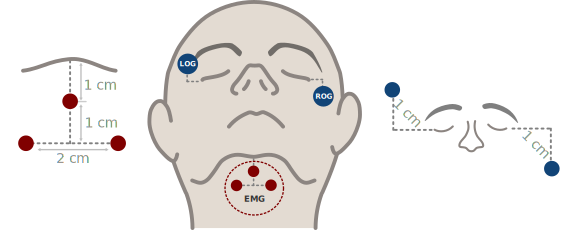
\includegraphics[width=\linewidth]
{./img_diagramas/emg_eog_v4.pdf}
\caption[Colocación de electrodos para el registro de electrooculograma y electromiograma]{Colocación de electrodos para el registro de electrooculografía en ambos ojos (LOG, ROG) y electromiografía (EMG). Las líneas punteadas son paralelas al eje medial, y las líneas discontinuas son perpendiculares al mismo. La línea de referencia para EMG inicia en el punto medial en la barbilla.}
\label{emg_eog}
\end{figure}



\begin{figure}
\centering
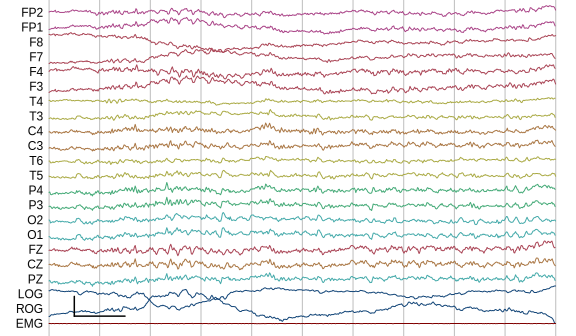
\includegraphics[width=\linewidth]
{./img_ejemplos/MJNN_epoca_stam.pdf}
\caption[Registro de polisomnograma durante sueño MOR]
{Registro de PSG durante sueño MOR. En el margen izquierdo se indica la derivación representada; aunque la mayoría corresponden al EEG, en la porción inferior se contempla al EOG y EMG.
Para más detalles sobre la ubicación de las derivaciones, ver el texto y la figura \ref{emg_eog}. Marca de calibración: vertical, 10 \mv, horizontal, 1 segundo.}
\label{ejemplos_mor}
\end{figure}

%%%%%%%%%%%%%%%%%%%%%%%%%%%%%%%%%%%%%%%%%%%%%%%%%%%%%%%%%%%%%%%%%%%%%%%%%%%%%%%%%%%%%%%%%%%%%%%%%%%
%%%%%%%%%%%%%%%%%%%%%%%%%%%%%%%%%%%%%%%%%%%%%%%%%%%%%%%%%%%%%%%%%%%%%%%%%%%%%%%%%%%%%%%%%%%%%%%%%%%

%\section{Relación entre deterioro cognitivo y sueño}
%
%Varios autores han reportado correlaciones, a nivel poblacional, entre el DCL y trastornos del sueño en adultos mayores \cite{Amer13,Miyata13,Reid06,Potvin12}.
%%
%%De forma enfática, la fase de sueño denominada MOR ha sido ampliamente relacionada con la consolidación de la memoria, así como con otras funciones cognitivas 
%%\cite{Fishbein1971,Fishbein1977,Lucero1970,Pearlman1971,Pearlman1974,Smith1991,corsi15}.
%
%El sueño MOR se ha asociado durante mucho tiempo con las funciones cognitivas \cite{Corsi1983}. 
%%
%El sueño MOR desempeña un papel en la consolidación de la memoria 
%\cite{Lucero1970, Fishbein1971, Fishbein1977, Pearlman1971, Pearlman1973, Pearlman1974, Smith1991,corsi15}.
%%
%Después de tareas complejas, hay reactivaciones de circuitos neuronales durante el sueño MOR \cite{Louie}. 
%%
%%La Potenciación a Largo Plazo (LTP) solo ocurre durante la vigilia y el sueño MOR, y, dependiendo de su fase theta del hipocampo, la LTP puede mejorarse o inhibirse \cite{Pavlides1988}.
%%
%El sueño MOR mejora la memoria y los procesos de atención mediante las entradas colinérgicas \cite{Braun1997} a través de la vía pontina \cite{Datta2004} y las estructuras del basales del cerebro anterior \cite{Blake}. 
%%
%Durante el envejecimiento normal y especialmente durante el envejecimiento patológico, los procesos de atención y memoria se vuelven más vulnerables, y las neuronas colinérgicas son las más afectadas \cite{Schliebs11}. 
%%
%%El envejecimiento afecta a varias estructuras anatómicas que resultan en la pérdida de un eje dendrítico en las neuronas corticales que muestran una degradación en su complejidad fractal estructural \cite{Lipsitz}.
%
%Se ha encontrado, por ejemplo, correlaciones entre el DCL en adultos mayores con la \textit{presencia} de ciertos tipos de ondas cerebrales \cite{babiloni13,prichep94,prichep06}.
%%
%%Sin embargo, otros estudios sugieren que el EEG durante el sueño es un mejor predictor del DCL [buscar y citar Baryet ??].
%%
%%El sueño MOR mejora la memoria y los procesos de atención mediante las entradas colinérgicas \cite{Braun} a través de pontine \cite{Datta2004} y las estructuras del basales del cerebro anterior \cite{Blake}. 
%%
%%Durante el envejecimiento normal y especialmente durante el envejecimiento patológico, los procesos de atención y memoria se vuelven más vulnerables, y las neuronas colinérgicas son las más afectadas \cite{Schliebs11}. 
%%
%%El envejecimiento afecta a varias estructuras anatómicas que resultan en la pérdida de un eje dendrítico en las neuronas corticales que muestran una degradación en su complejidad fractal estructural \cite{Lipsitz}.
%
%%Las causas inmediatas del DCL pueden rastrearse al deterioro en varias estructuras cerebrales.
%%
%Los procesos de atención y memoria dependen de circuitos colinérgicos (grupos de neuronas cuyo principal transmisor es la acetilcolina); estos circuitos son propensos a degradación estructural durante el envejecimiento, y en mayor medida si es un envejecimiento patológico \cite{Schliebs11}.
%%
%Cabe destacar que los circuitos colinérgicos son activados de forma importante durante el sueño, particularmente en la fase deniminada MOR \cite{Braun1997}.
%
%%El EEG durante el sueño MOR ha demostrado ser un indicador del DCL en adultos mayores. 
%%
%Se ha reportado una mayor potencia absoluta y relativa en frecuencias lentas para regiones laterales \cite{Brayet16} y una menor atonía muscular \cite{Chen} para adultos mayores con DCL, respecto a individuos sanos.
%
%Los estudios anteriores han incluido análisis del EEG o del EMG, pero el EOG no se ha considerado como un posible marcador del DCL. 
%%Los tres indicadores de sueño MOR aparecen generalmente en orden consecutivo. Al ingresar a esta etapa, los husos y las ondas lentas de alta amplitud están ausentes, el EEG tiene abundantes frecuencias beta y gamma \cite{SteriadeIntracortical1996,Llinas}, hay una abrupta pérdida de voltaje que ocurre en un intervalo menos de 2 segundos \cite{Rosales-Lagarde2009}, y, luego, aparcen los movimientos oculares (MOR) característicos \cite{AASM07}.
%%\cite{Aserinsky,AASM07,Rechtshaffen1968}.
%
%%En concreto se utilizarán registros de varias señales electrofisiológicas --electroencefalograma (EEG), electrooculograma (EOG) y electromiograma (EMG)--, técnica conocida como polisomnografía (PSG)\footnote{La 
%%PSG puede contener otro tipo de señales como electrocardiograma, niveles de oxígeno en la sangre, 
%%esfuerzo respiratorio, movimiento de las piernas, entre otras}, obtenidas durante 
%%etapas específicas en el sueño del paciente.
%%%ANADÏ ESTO, checar para qué figura queda, porque debe especificarse que comunmente en la PSG se registran 2 electrodos, C3 y C4, emg y ojos. Sin embargo, como el objetivo es conocer la actividad eléctrica cerebral de más regiones, se colocaron 19 electrodos en la cabeza de cada paciente, dispuestos según el sistema 10/20. ESTO DEBE ESTAR EN EL PIE DE FIGURA CORRESPONDIENTE. NO ME ACUERDO SI ESTÁ O NO, PERO FUE QUE NOS PIDIERON QUE EXPLICARAS MÁS...Y LO DE LAS OREJAS CORTOCIRCUITADAS. CITA AL MANUAL DE NIEDERMEYER

%%%%%%%%%%%%%%%%%%%%%%%%%%%%%%%%%%%%%%%%%%%%%%%%%%%%%%%%%%%%%%%%%%%%%%%%%%%%%%%%%%%%%%%%%%%%%%%%%%%
%%%%%%%%%%%%%%%%%%%%%%%%%%%%%%%%%%%%%%%%%%%%%%%%%%%%%%%%%%%%%%%%%%%%%%%%%%%%%%%%%%%%%%%%%%%%%%%%%%%

\section{Relación entre deterioro cognitivo y sueño}
\label{sec:pdcl_sueno}

Varios autores han reportado correlaciones, a nivel poblacional, entre el DCL y trastornos del sueño en adultos mayores \cite{Amer13,Miyata13,Reid06,Potvin12}.

El sueño MOR se ha asociado durante mucho tiempo con las funciones cognitivas \cite{Corsi1983}. 
%
El sueño MOR desempeña un papel en la consolidación de la memoria 
\cite{Lucero1970, Fishbein1971, Fishbein1977, Pearlman1971, Pearlman1973, Pearlman1974, Smith1991,corsi15}.
%
Después de tareas complejas, hay reactivaciones de circuitos neuronales durante el sueño MOR \cite{Louie}. 
%
El sueño MOR mejora la memoria y los procesos de atención mediante las entradas colinérgicas \cite{Braun1997} a través de la vía pontina \cite{Datta2004} y las estructuras del basales del cerebro anterior \cite{Blake}. 
%
Durante el envejecimiento normal y especialmente durante el envejecimiento patológico, los procesos de atención y memoria se vuelven más vulnerables, y las neuronas colinérgicas son las más afectadas \cite{Schliebs11}. 

Se ha encontrado, por ejemplo, correlaciones entre el DCL en adultos mayores con la \textit{presencia} de ciertos tipos de ondas cerebrales \cite{babiloni13,prichep94,prichep06}.

Los procesos de atención y memoria dependen de circuitos colinérgicos (grupos de neuronas cuyo principal transmisor es la acetilcolina); estos circuitos son propensos a degradación estructural durante el envejecimiento, y en mayor medida si es un envejecimiento patológico \cite{Schliebs11}.
%
Cabe destacar que los circuitos colinérgicos son activados de forma importante durante el sueño, particularmente en la fase deniminada MOR \cite{Braun1997}.

Se ha reportado una mayor potencia absoluta y relativa en frecuencias lentas para regiones laterales \cite{Brayet16} y una menor atonía muscular \cite{Chen} para adultos mayores con DCL, respecto a individuos sanos.

%%%%%%%%%%%%%%%%%%%%%%%%%%%%%%%%%%%%%%%%%%%%%%%%%%%%%%%%%%%%%%%%%%%%%%%%%%%%%%%%%%%%%%%%%%%%%%%%%%%
%%%%%%%%%%%%%%%%%%%%%%%%%%%%%%%%%%%%%%%%%%%%%%%%%%%%%%%%%%%%%%%%%%%%%%%%%%%%%%%%%%%%%%%%%%%%%%%%%%%
%%%%%%%%%%%%%%%%%%%%%%%%%%%%%%%%%%%%%%%%%%%%%%%%%%%%%%%%%%%%%%%%%%%%%%%%%%%%%%%%%%%%%%%%%%%%%%%%%%%
%%%%%%%%%%%%%%%%%%%%%%%%%%%%%%%%%%%%%%%%%%%%%%%%%%%%%%%%%%%%%%%%%%%%%%%%%%%%%%%%%%%%%%%%%%%%%%%%%%%